\subsubsection{Hadronisation mechanisms for c and b quarks}
\label{sec:HFhadro1}

%Brief intro to fragmentation vs recombination
%describe recombination implementations with references, also statistical hadronisation?
%effects of hadronisation on yields, pT spectrum, v2
%Available RHIC and LHC data (no figures)
%Discuss also Bs and Bc, see e.g. arXiv:hep-ph/0004041

The hadronisation mechanisms belong to the non-perturbative domain of QCD and a
first-principle description of these processes is still missing, for both light and heavy flavours.
However, from the study of charm dynamics in nucleus--nucleus collisions in the last decade
there is a general consensus that the details of hadronisation have a large effect on both the heavy-flavour observables 
$\RAA$ and $\vtwo$~\cite{Dong:2018ntm,Rapp:2018qla,Scardina:2017ipo}.
This section introduces 
the two main microscopic hadronisation mechanisms for the production of heavy-flavour hadrons: fragmentation and coalescence (also denoted as recombination).
Fragmentation is one of the most common approaches for the calculation of inclusive hadron production and it is appropriate
for high-momentum partons emerging
from initial hard processes, where high-momentum quarks fragment directly and independently into high-momentum hadrons. Independent fragmentation has also been widely applied at low momentum in $\rm e^+e^-$, ep and pp collisions.
On the other hand, coalescence is expected to dominate in the low-momentum regime in nucleus--nucleus collisions, where partons are abundant and heavy quarks
can hadronise by recombination with light quarks~\cite{Fries:2008hs}. Recent measurements at the LHC indicate that fragmentation may not be sufficient to 
describe charm quark hadronisation at low momentum in pp and p--Pb collisions, at least
for what concerns baryon production~\cite{Acharya:2017kfy,Acharya:2017lwf}.

The hadron momentum spectra produced by heavy-quark fragmentation is given by:
\begin{equation}
\frac{{\rm d}N_{\rm had}}{{\rm d}^{2}\pT\,{\rm d} y}=\sum \int {\rm d} z \frac{{\rm d} N_{\rm fragm}}{{\rm d}^{2}\pT\, {\rm d} y} \frac{D_{\rm had/Q}(z,Q^{2})}{z^{2}} 
\label{Eq:frag}
\end{equation}
where $z=p_{\rm had}/p_{\rm Q}$ is the fraction of quark momentum carried by the hadron and $Q^2=(p_{\rm had}/2 z)^2$ 
is the momentum scale for the fragmentation process.

In the basic coalescence model developed in Refs.~\cite{Greco:2003mm,Greco:2003vf,Fries:2003kq,Fries:2003vb,Oh:2009zj,Minissale:2015zwa,Plumari:2017ntm}
the spectrum of heavy-flavour hadrons formed by coalescence of heavy-light quarks can be written as
\begin{equation}
\label{eq-coal}
\frac{{\rm d}^{2}N_{\rm had}}{{\rm d}\pT^{2}}
= g_{\rm had} \int \prod^{n}_{i=1} \frac{{\rm d}^{3}p_{i}}{(2\pi)^{3}E_{i}} p_{i} 
\cdot {\rm d}\sigma_{i}  \cdot f_{q_i}(x_{i}, p_{i})  
f_{\rm had}(x_{1}...x_{n}, p_{1}...p_{n})\, 
\delta^{(2)} \left(p_{\rm T,had}-\sum^{n}_{i=1} p_{{\rm T},i}\right)
\end{equation}
where ${\rm d}\sigma_{i}$ denotes an element of a space-like hypersurface and $f_{q_i}$ are the quark (antiquark)
phase-space distribution functions for $i$-th quark (antiquark), while $g_{\rm had}$ is the statistical factor
to form a colourless hadron from quarks and antiquarks with spin 1/2.

Hadronisation via coalescence leads to a modification of the relative abundance of the
various heavy-flavour hadron species produced. 
The most striking effect is an enhancement of the baryon-to-meson ratios for heavy-flavour hadrons.
First studies of these ratios~\cite{Oh:2009zj,Plumari:2017ntm} indicated a significant change in the relative abundances of the heavy-flavour hadron species, and in particular a ratio of $\PGLc/\PDzero$ close to unity, which
is nearly an order of magnitude larger than what predicted by the fragmentation
process implemented in the PYTHIA event generator. 
This value is also much larger than the
prediction of the statistical hadronisation model~\cite{Andronic:2007zu}, in which the hadronisation occurs by recombination of an equilibrated system of quarks and the hadron abundances are mainly determined by their masses.
In addition, hadronisation via coalescence in a strangeness-rich Quark-Gluon Plasma is predicted to lead to a large enhancement in the production of strange heavy-flavour hadrons, like $\PDs$ and $\PBs$~\cite{Kuznetsova:2006hx,He:2014cla,Song:2015ykw}.
Hints of an enhancement of the $\PDs/\PDzero$ and $\PGLc/\PDzero$ ratios in nucleus--nucleus collisions have recently been reported by ALICE at the LHC~\cite{Acharya:2018hre,Peng:2018pwj} and by STAR at RHIC~\cite{Radhakrishnan:2018xxx}.

The hadronisation by coalescence plus fragmentation also affects the $\pT$ distribution  of heavy-flavour hadrons. For D mesons the effect can be roughly seen as a
shift in $\pT$ of about 1.0--1.5~\UGeVc in the region of $\pT$ of 1.5--6~\UGeVc, resulting in a
significant enhancement of $\RAA(\pT)$. The degree of these enhancements for D meson, however, is
significantly different  among the different implementations of the hadronisation
by coalescence and it is nearly unknown for heavy-flavour baryons, like \PGLb and \PGLc.

Finally, the coalescence process leads to a significant enhancement of the $\vtwo(\pT)$ in the
intermediate $\pT$ region that, for D mesons, amounts to about 20--40\% depending on the
specific modelling. The \PGLc is expected to acquire instead a much 
larger enhancement of at least a factor of two for the $\vtwo$. Therefore, a combined measurement of the
$\PGLc/\PDzero$ and $\rm \Lambda_b/B$ ratios and of the baryon elliptic flow would impose strong constraints
on the hadronisation mechanism and lead to a better determination of the diffusion transport coefficient of heavy quarks (see Section~\ref{sec:HFhadro3}).

\subsubsection{Measurement performance studies (ALICE and CMS)}
\label{sec:HFhadro2}


Simulation studies for the measurement of the $\PDs$, \PGLc and \PGLb
production were carried out by the ALICE Collaboration~\cite{Abelev:1625842} and are updated in the present document. A projection of the performance for the $\PBs$ meson by the CMS Collaboration is also reported~\cite{CMS-PAS-FTR-17-002}. The $\PDs$, \PGLc and \PGLb ($\to\Lambda_c\pi$) reconstruction strongly benefits from the improved track spatial resolution of the ALICE Inner Tracking System Upgrade, because they have small mean proper decay lengths (e.g.\,about 60~$\mu$m for \PGLc)
and large combinatorial backgrounds. The \PGLc, \PGLb and $\PBs$, in particular, require very large integrated luminosities, because the decay branching ratios are very small (e.g.\,about $3\times 10^{-4}$ for $\rm \Lambda_b\to\Lambda_c(\to pK\pi)\pi$) and the combinatorial background is very large, in case for the \PGLc, which has a small separation from the interaction vertex and lower invariant-mass than the b-hadrons. In~\cite{CMS-PAS-FTR-17-002} it has been shown that the statistical uncertainty in the lowest accessible $\pt$ intervals for these hadrons would increase above 20--30\% with integrated luminosity significantly lower than 10~nb$^{-1}$.

Figure~\ref{fig:HFDsBs} shows the performance for the $\RAA$ of $\PDs$ (left) and $\PBs$ (right), compared with the corresponding non-strange mesons. The predicted difference between the $\rm D^0$ and $\PDs$ $\RAA$ will be measured very precisely and the difference in the beauty sector could be observed with a significance of about 3\,$\sigma$.
The measurements were studied only for $p_{\rm T}>2$ and 8~GeV$/c$, respectively, but an extension to lower $\pt$ is considered within reach.

\begin{figure}[!t]
\centering
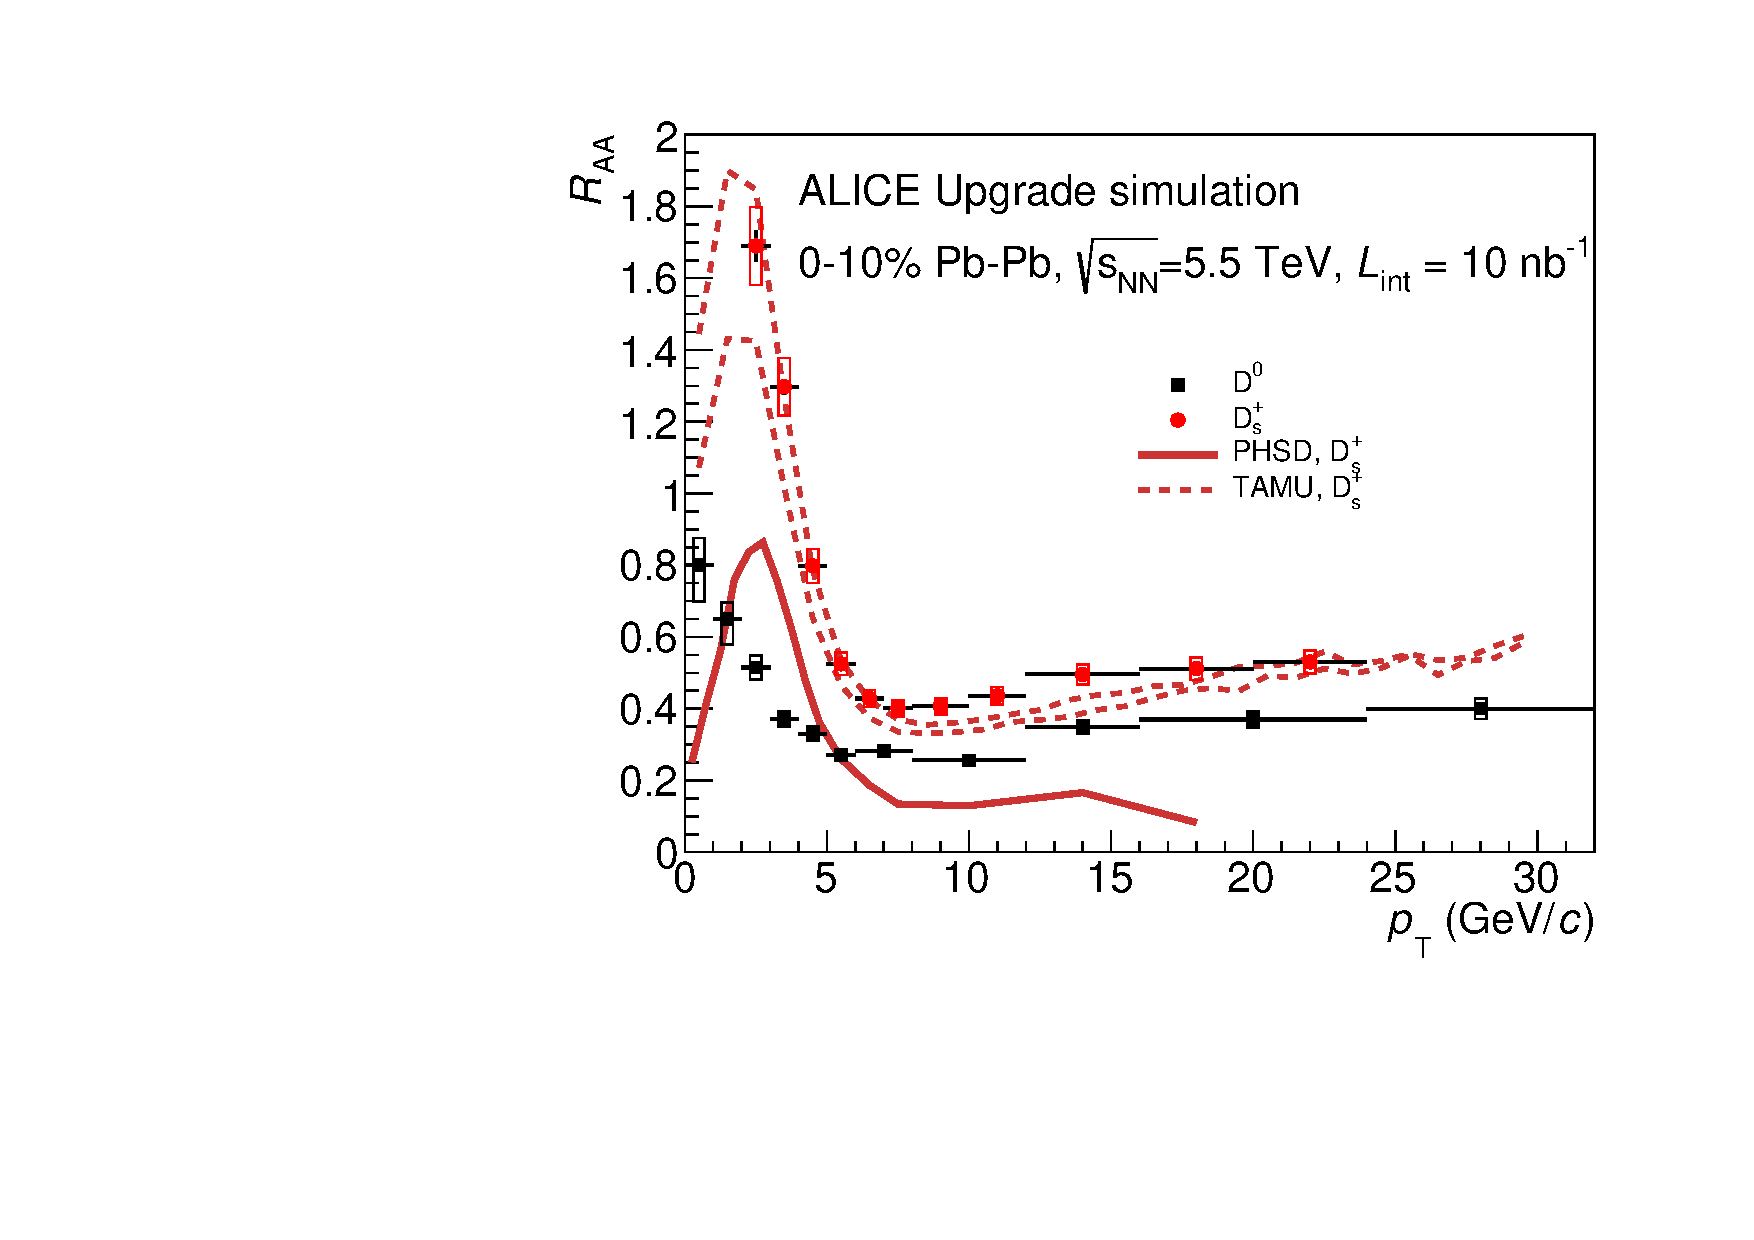
\includegraphics[width=0.55\textwidth]{hf/figures/ALICEUpgrade_D0_Ds_RAA_YR.pdf}
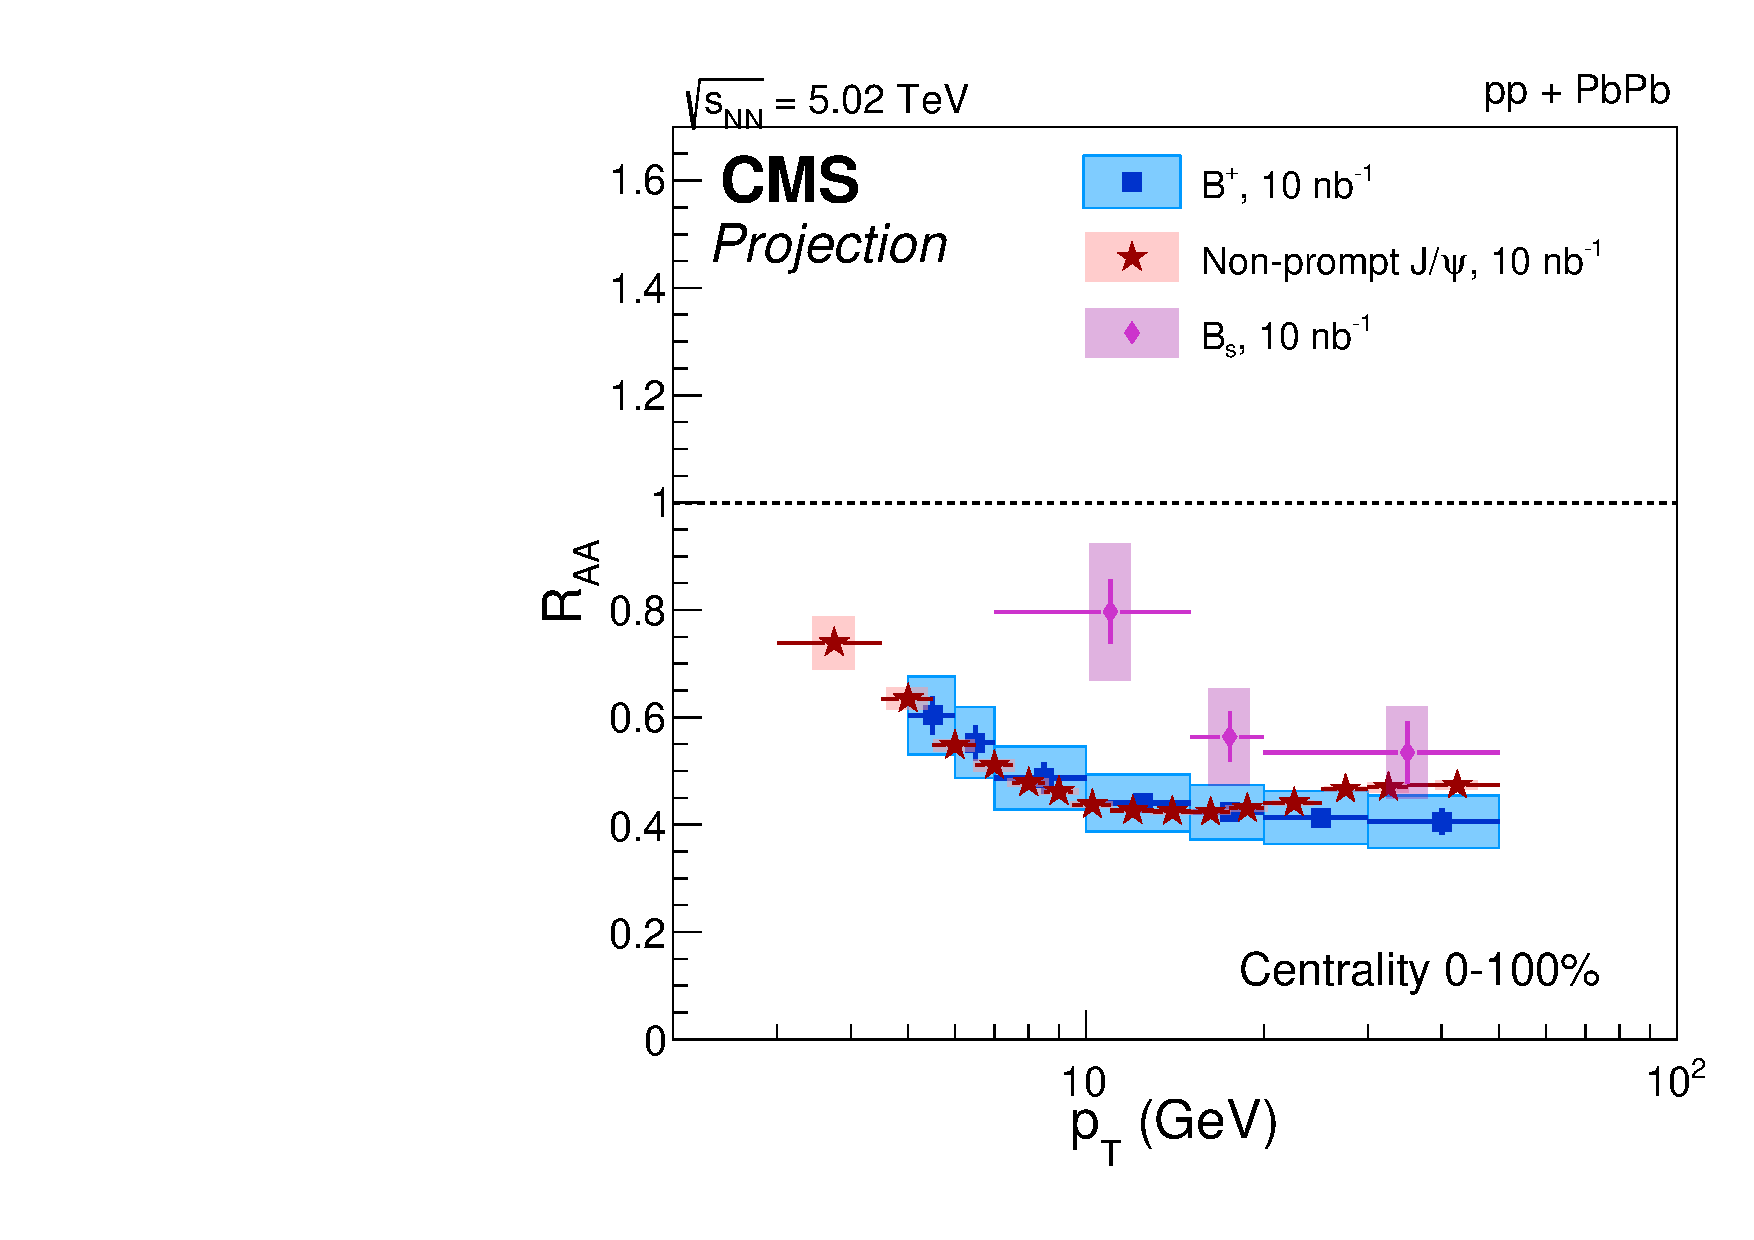
\includegraphics[width=0.44\textwidth]{hf/figures/CMS_B_Bs_RAA.pdf}
\caption{Measurement performance projections for the nuclear modification factor  $\RAA$ of $\PDs$ (left) and $\PBs$ (right) mesons in \PbPb collisions ($\Lint=10~\invnb$). The ALICE study for $\PDs$ is based on full simulation~\cite{Abelev:1625842}. The CMS projection is based on scaling of uncertainties from existing measurements~\cite{CMS-PAS-FTR-17-002}.}
\label{fig:HFDsBs}
\end {figure}

\begin{figure}[!t]
\centering
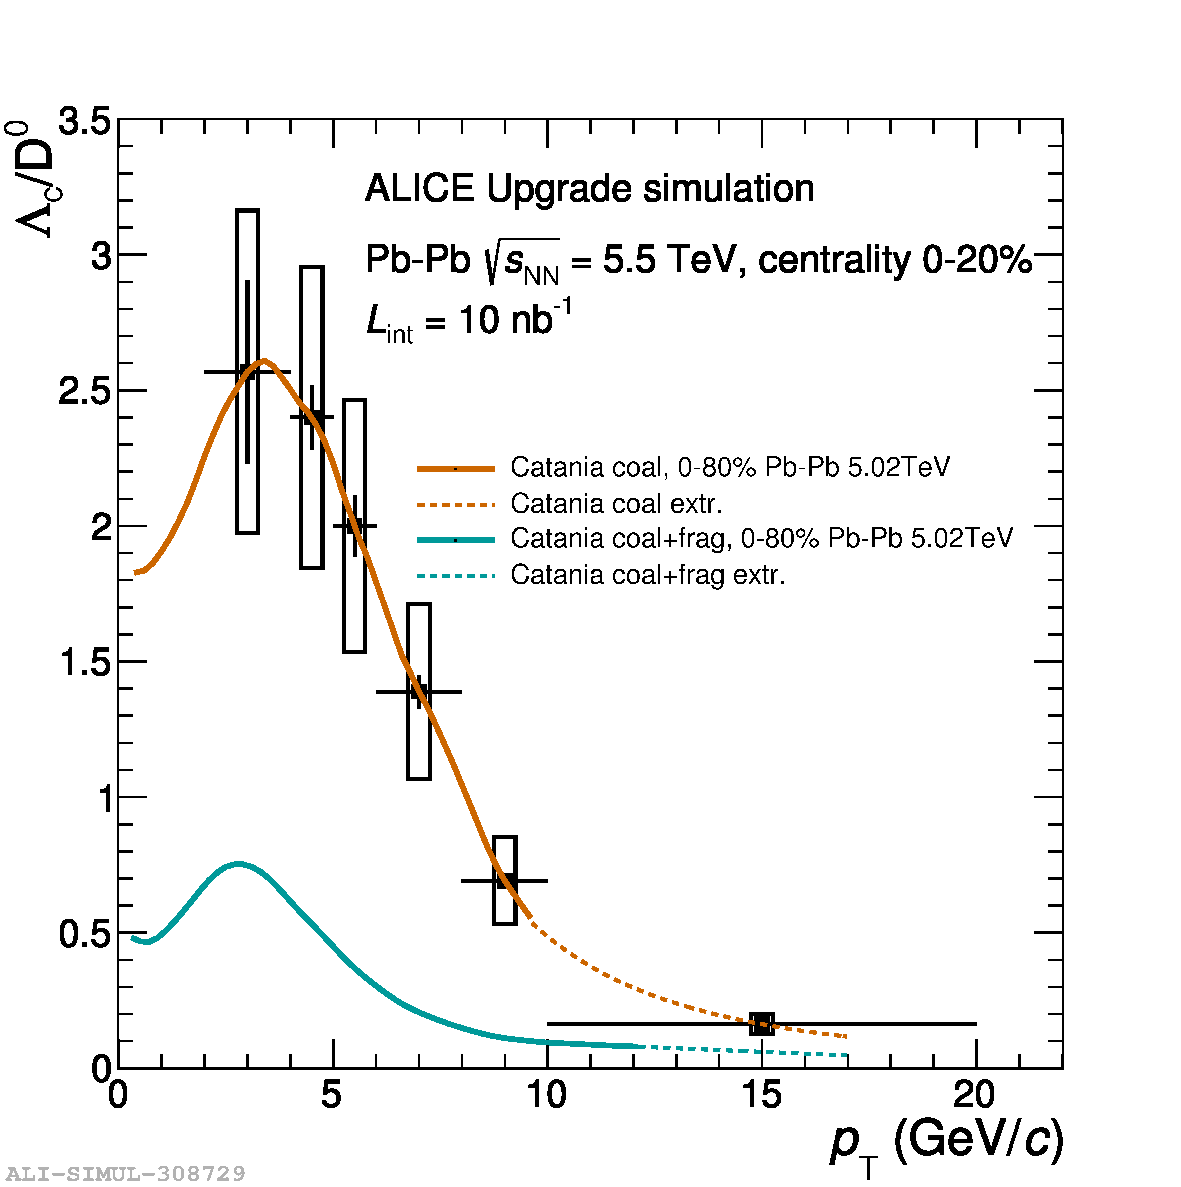
\includegraphics[width=0.49\textwidth]{hf/figures/ALICE_LcOverD_YR.pdf}
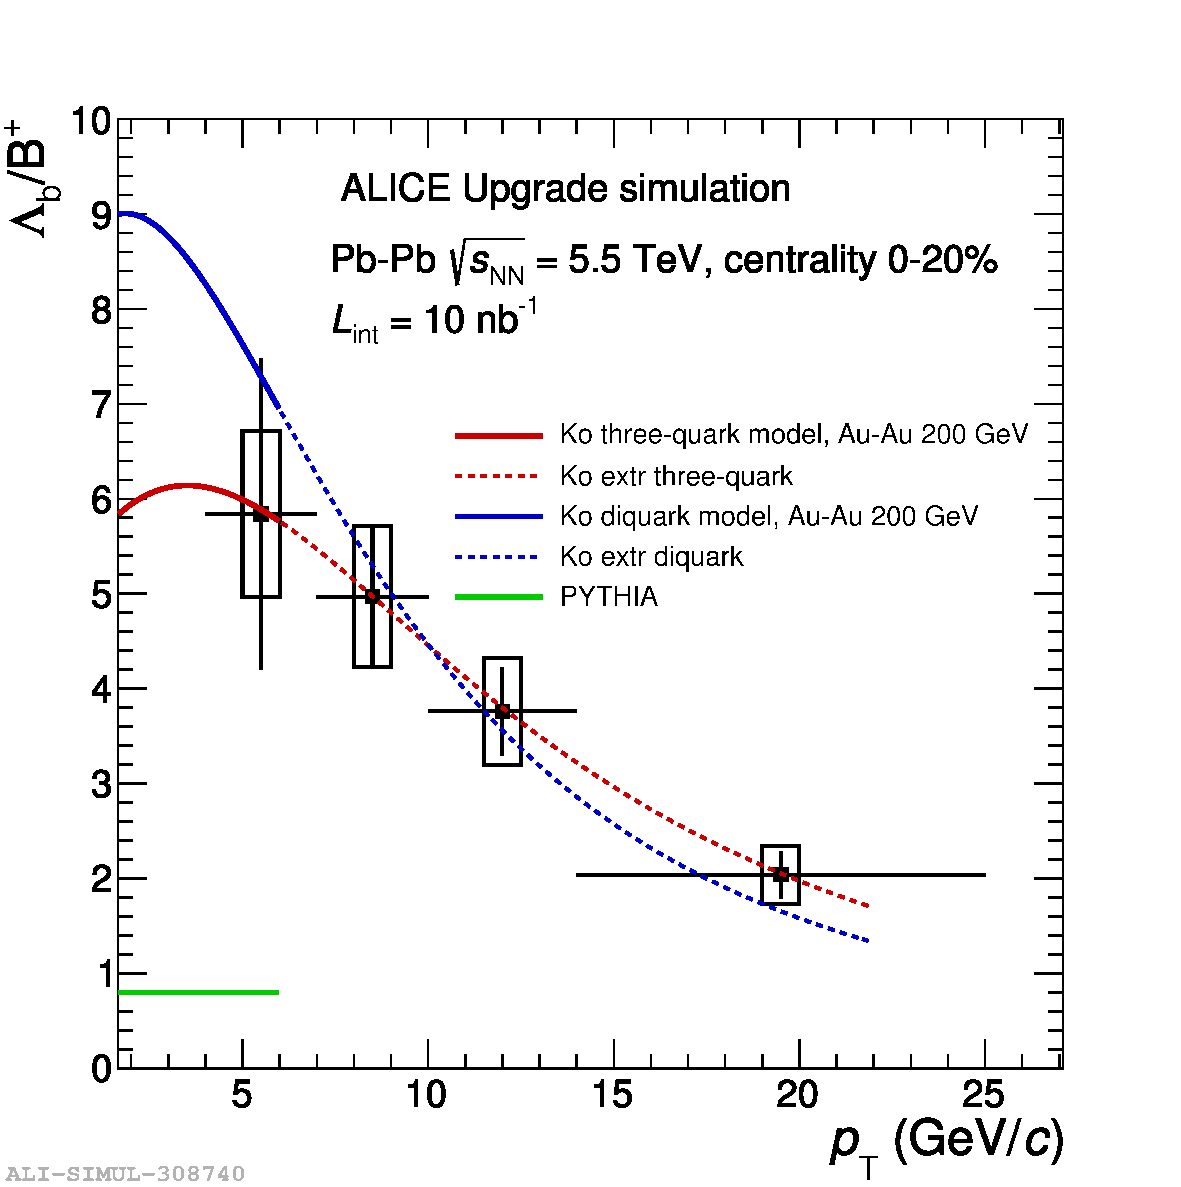
\includegraphics[width=0.49\textwidth]{hf/figures/ALICE_LbOverB_YR.pdf}
\caption{ALICE measurement performance for the $\Lambda_c/D^0$ (left) and $\Lambda_b/B^+$ ratios in central \PbPb collisions ($\Lint=10~\invnb$), based on studies from~\cite{Abelev:1625842}.}
\label{fig:HFLcLb}
\end {figure}

Figure~\ref{fig:HFLcLb} shows the performance for the charm and beauty baryon-to-meson ratios as they can be measured by ALICE with $\Lint=10~\invnb$ ~\cite{Abelev:1625842}. The measurements are compared with predictions based on various mechanisms for heavy-quark recombination in the medium~\cite{Plumari:2017ntm,Oh:2009zj}.
Figure~\ref{fig:RAAv2.v2charm} (right) shows the performance for the elliptic flow coefficient $\vtwo$ of $\rm D^0$, $\PDs$ and \PGLc 
in semi-central \PbPb collisions~\cite{Abelev:1625842}. The precision of the $\PDs$ $\vtwo$ should be sufficient to enable a significant comparison with $\rm D^0$ and with model calculations, in which the 
observable is found to be sensitive to the interactions of $\rm D$ mesons in the hadronic phase that characterises the late stages of the collision~\cite{He:2014cla}. 
Both measurements cannot be extended to the very-low-momentum region, where the separation of the heavy-flavour secondary vertex from the primary vertex is small.  
This limitation motivates studies for a further improvement of the ALICE inner tracker during LS3~\cite{ALICEITS3}.  A more precise measurement would open the possibility to test in the charm sector some features at present only observed for the $\vtwo$ of light-flavour hadrons: the mass scaling at low $\pt$ and 
the baryon--meson grouping at high $\pt$.

% THIS FIGURE IS NOW IN THE PREVIOUS SECTION
%\begin{figure}[ht]
%\centering
%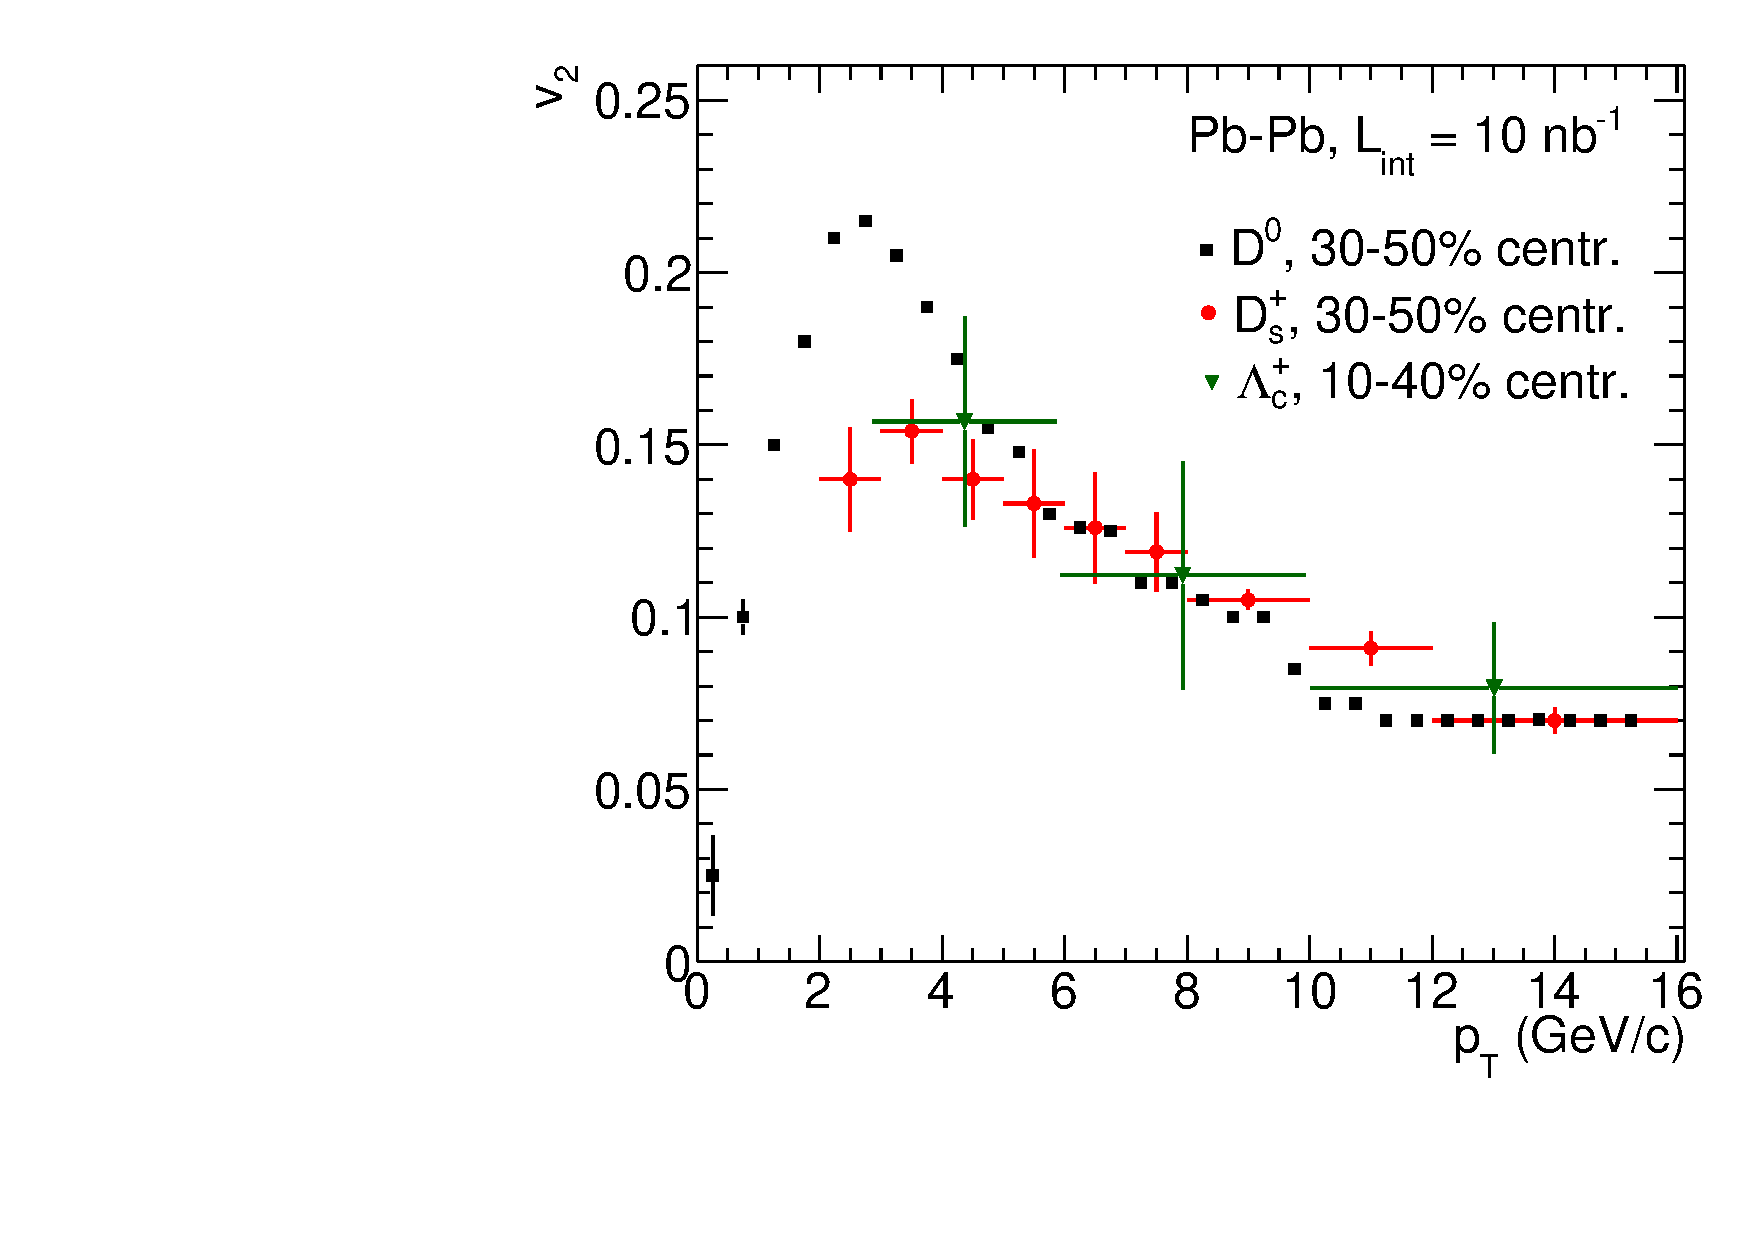
\includegraphics[width=0.40\textwidth]{hf/figures/D0DsLc_v2_TDR.pdf}
%\caption{ALICE measurement performance projections for the elliptic flow coefficient $\vtwo$ of $D^0$, $D_s$ and $\Lambda_c$ in \PbPb collisions ($\Lint=10~\invnb$)~\cite{Abelev:1625842}.}
%\label{fig:D0DsLcv2}
%\end {figure}



\subsubsection{Constraining HF hadronisation}
\label{sec:HFhadro3}

%Discuss sensitivity of expected measurements to recombination fraction and parameters (use Catania model as example)
%Discuss impact on extraction of HQ diffusion coefficient

\begin{figure}[!hb]
\begin{center}
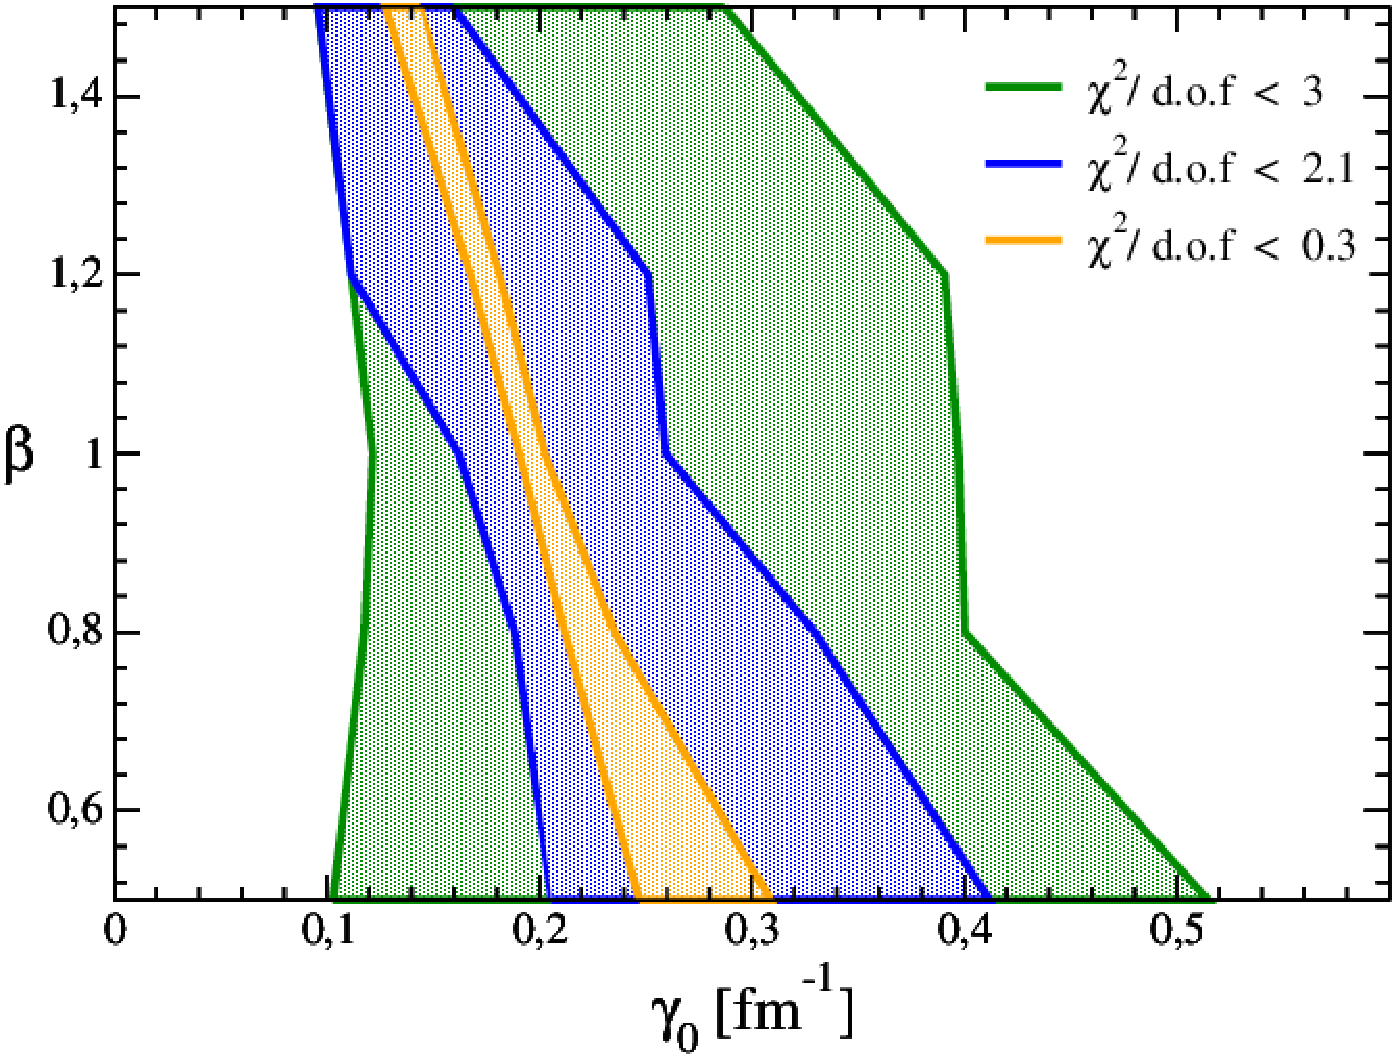
\includegraphics[width=0.49\textwidth]{hf/figures/chi2_vers2.pdf}
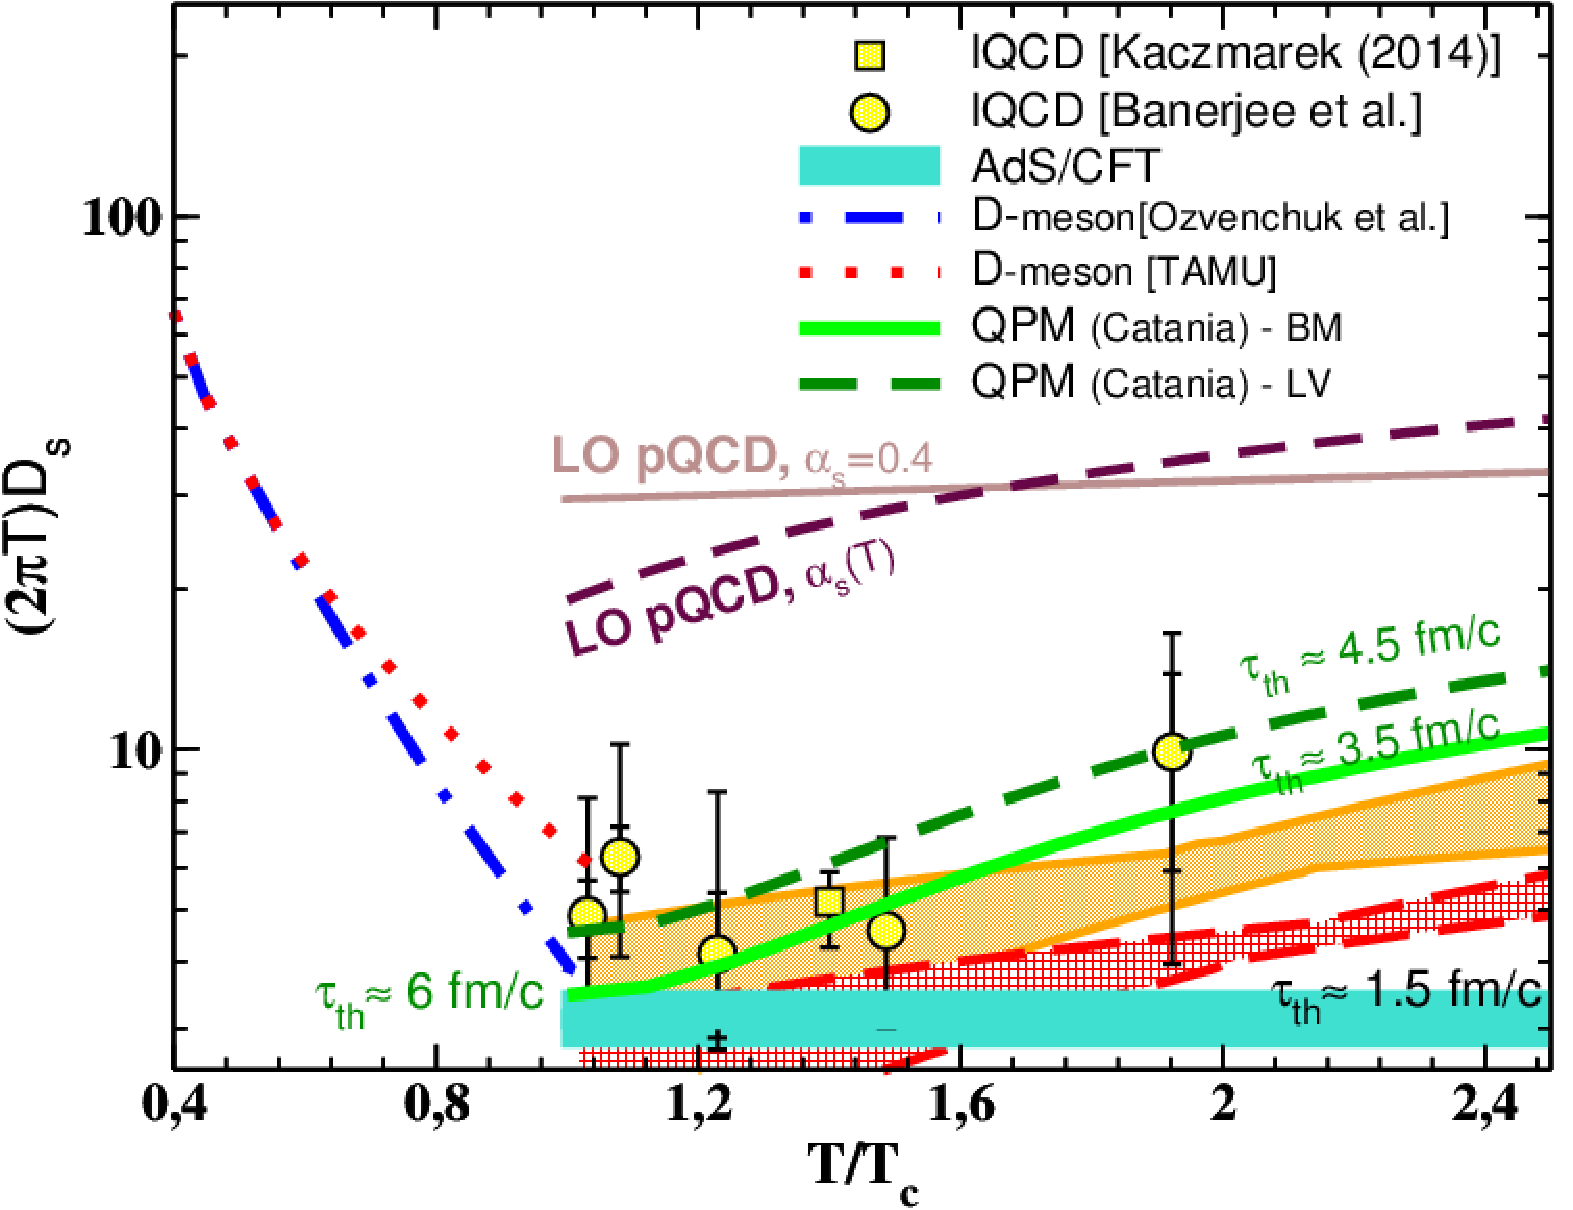
\includegraphics[width=0.49\textwidth]{hf/figures/Ds_lQCD_CHI2_COAL-FRAGM.pdf}
\end{center}
\caption{Illustration of charm diffusion coefficient $2\pi T D_s$ estimate from D meson $\RAA$ data using different hadronisation assumptions in the Catania model~\cite{Das:2015ana,Das:2013kea}. Left: $\chi^2/d.o.f$ in the ($\gamma_0$,$\beta$)  parameter space for the case with only fragmentation.
Right: diffusion coefficient as a function of temperature. The orange band refers to fit 
with fragmentation only, the red band to the fit with coalescence plus fragmentation.}
\label{Fig:CHI2}
\end{figure}


The hadronisation mechanism of heavy quarks is important for the description of the measured
heavy-flavour $\RAA$ and $\vtwo$ at RHIC and LHC energies. In particular, it has been recognized that recombination
play a dominant role in describing simultaneously both D meson $\RAA$ and $\vtwo$~\cite{Gossiaux:2008jv,He:2011qa,Scardina:2017ipo}.
Moreover, as discussed in Section~\ref{sec:HFhadro1}, the charm baryon-to-meson ratio $\PGLc/\PDzero$ measured at RHIC and LHC is not consistent with a fragmentation only scenario~\cite{Oh:2009zj,Plumari:2017ntm}.
Therefore, a combined study including also the heavy baryon-to-meson ratio provides further
information to solve the ambiguity on the
recombination fraction. As such it is important to investigate the different sensitivity
of different observables to the
recombination fractions described in Section~\ref{sec:HFhadro1}.
To estimate how different model implementations of the hadronisation mechanisms can affect the extraction of the charm quark diffusion coefficient $2\pi T D_s$,
a global quantitative $\chi^2$ analysis was carried out by comparing experimental data on the D meson $\RAA$ with theoretical
results obtained using the Fokker-Planck equation under a standard bulk medium evolving
hydrodynamically with $\eta/s=0.1$~\cite{Plumari:2015cfa,Ruggieri:2013ova}.
The model developed in~\cite{Das:2015ana,Das:2013kea} with diffusion and drag
coefficients related by the fluctuation-dissipation theorem was used, considering two different
implementations of the hadronisation process: one using only fragmentation of charm quarks to D mesons (with the Peterson function)
and another one including a hybrid hadronisation by coalescence plus fragmentation~\cite{Plumari:2017ntm,Scardina:2017ipo}.
For the estimate of the temperature dependence of $2\pi T D_s$, a schematic model in which the
drag coefficient is parametrized as $\gamma=\gamma_0 (T/T_{c})^{\beta}$ was used. For illustration, the two parameters $\gamma_0$ and $\beta$ were determined by minimizing the
$\chi^2/d.o.f$ of the model with respect to the measured D meson $\RAA$. The exercise could in principle be repeated using both $\RAA$ and $\vtwo$. 
The spatial diffusion coefficient is directly related to
the drag coefficient by $D_s=T/(M\cdot\gamma)$, where $M$ is the charm quark mass.
The left panel of Fig.~\ref{Fig:CHI2} shows the parameter space ($\gamma_0,\, \beta$) for the fragmentation only case and for three range of the reduced $\chi^2$. The right
panel shows the spatial diffusion coefficient $2\pi T D_s(T)$ estimated from the fit to the data ($\chi^2/d.o.f \leq 0.3$ range): the orange band corresponds to the fragmentation only 
results and the red band to the fragmentation plus coalescence results. Clearly, an optimal estimate of the diffusion coefficient requires an accurate description of the hadronisation mechanism in the model.



